\chapter{Introduction}
\label{ch:intro}

% This is the introduction. It should describe your completed senior thesis work, including the overall aims and the background motivating your research. Whenever possible, you should use one or more concrete examples
% and technical diagrams. 

% It is often useful and necessary to separate the introduction into multiple section. Several possible sections are proposed below, you can use these or distribute your introductory text into sections in another way. 

\section{Motivation} 
\label{sec:motivation}

% This section should include a statement of the problem, the overall aims, and the background motivating your research. Whenever possible, you should use one or more concrete examples
% and technical diagrams.
Pathfinding algorithms for autonomous field robots do not often take into account the energy cost of the path subsections when determining which route to traverse. This leads to wasted battery in robots where operational time is crucial to their intended purpose, like bomb disposal robots or search and rescue robots.\cite{henkel2016energy}. Robots that operate on battery and are sent into dangerous situations need to be able to operate for long enough that they can complete their mission without needing to come back and recharge. Many robots, such as bomb disposal robots, tend to waste power when traveling up inclines or on rough terrain, and this wasted power leads to a lower total operational time for the robot\cite{dasgupta2015comrade}.
\par
Longer operational time for field robots is a necessity, because in certain situations it can mean life or death for a person in a crisis. In search and rescue operations, such as in the case of natural disasters, people may be trapped and in imminent danger. The longer a robot can operate, the more likely it is that said person in danger can be located and/or rescued successfully. Another type of field robot that this affects is a bomb disposal robot. In post-conflict zones, the longer bombs are left, the more dangerous they become to the people in the region. Enabling each robot in the system to operate for longer means that in a given search, the robots are likely to find more bombs/explosives and deal with them properly\cite{dasgupta2015comrade}.
\par
A number of considerations are important when it comes to solving this problem, such as some of the following\cite{henkel2016energy}:
\begin{enumerate}
    \item Motor Resistance
    \item Friction
    \item System Vibrations
\end{enumerate}
\par
These elements all contribute to potential wasted power, because the higher the Motor Resistance, the more power it takes to move the motor a set distance. The more friction the ground exerts, the less power is required to rotate the wheels. The more friction the ball-bearings have in the wheels, the harder it is for the wheels to turn and thus it will draw more power. If the system is vibrating, then the ground friction will vary and a number of other issues with the robot will arise\cite{henkel2016energy}.

%\section{Current State of the Art}
%\label{sec:stateofart}
\section{Goals of the Project}
\label{sec:goals}
This project implements a simulation system that takes the pathfinding algorithms from several different sources and compares them in terms of different relevant metrics to the operational time of autonomous field robots. The intended functionality is for users to be able to provide or select from a few pathfinding algorithms currently used in autonomous field robots, and then the system designed in this project runs each of them and provides an analysis of how long each took to run, how much battery power the robot would require to traverse the chosen path, and also how much memory the algorithm used while it was running.
\par
This system provides the user with information about which algorithm is best suited to the robot that they provide as parameters to the simulation, and the expected environment in which that robot will operate. Each pathfinding algorithm will likely have certain environment types or robot weights in which cases they will be more effective and battery efficient. This research may also lead to a general case where a certain algorithm will be more efficient in most cases.
\par
By using this system, choosing the most battery-efficient pathfinding algorithm for the expected environment or the robot becomes easier, and enhances the operation time of autonomous robots in critical roles like search and rescue operations or bomb disposal. After this project, the simulation program will be able to be expanded for use with different pathfinding algorithms beyond those used in this project, and also with more complex sets of parameters and evaluation metrics for each algorithm.
\par
In addition to the simulation system, a modified version of the A* algorithm has been created that takes battery life into account as a weighting factor when determining the shortest path. Using the analysis of the other algorithms based on energy consumption, this new algorithm chooses a more energy efficient path than that of the other algorithms that do not inherently assess the energy cost of a given path. 

\section{Overview of Methods}
This project has created a "simulation room" of sorts in which a user is able to enter a pathfinding algorithm mathematically as a function, and compare it to other added robot pathfinding algorithms. This comparison is based on a variety of factors, such as the battery cost of the chosen route, the time it took to calculate the chosen route, and the amount of memory that was used during the calculation. The general process of using the simulation tool is outlined in Figure \ref{fig:Usage}.
\begin{figure}[H]
    \centering
    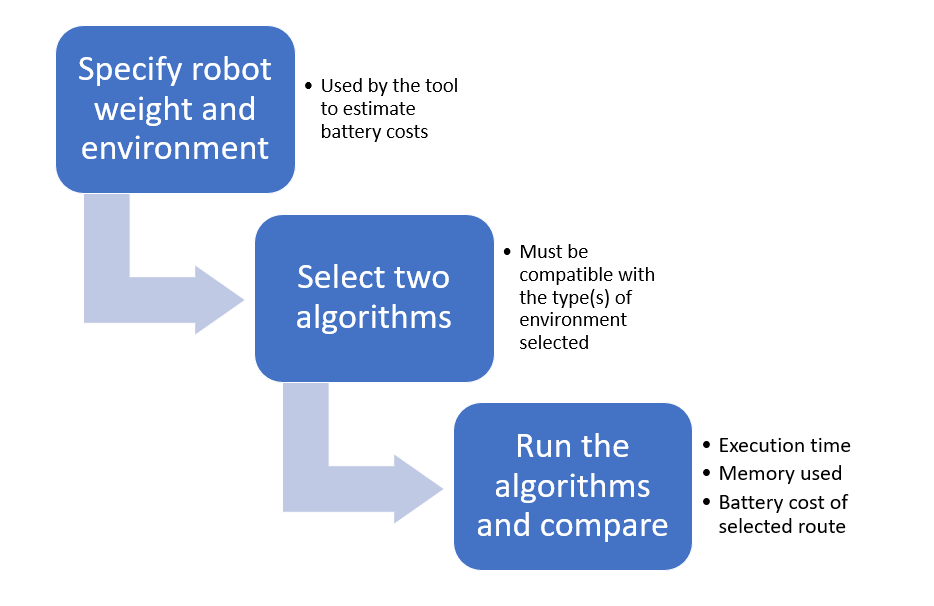
\includegraphics[width=5in]{../images/ProposalMethodFlowchart}
    \caption{The process for using the simulation tool}
    \label{fig:Usage}
\end{figure}
Each algorithm is able to be assessed based on the amount of time it takes to run the algorithm, how much memory it consumed, and how much battery power the calculated route will take to execute. Each of these metrics will be able to be used by robot designers to determine which algorithm best suits their needs for the robot that they are designing.
\par
This project has been written in Python due to the large number of available libraries and the general ease of use of the language. Numpy \cite{numpy_2021} has been used in the implementations of the various pathfinding algorithms, and the integrated system libraries were useful for tracking metrics such as the time it took to execute the algorithms and how much memory they use.
\par
As this approach purely looks at the performance of these pathfinding algorithms via a software approach and the physics used, the battery consumed statistic may be inaccurate when compared to a real robot using those pathfinding algorithms. Certain robot designs would likely require different amounts of battery power for a given route, meaning that in the future this system will likely need to be able to support different physics calculations based on varying numbers of drive motors or robot weights.
\par
This project assumes that each pathfinding algorithm will take either similar input or input that will be able to be derived from the simulated environment that will be created mathematically for traversal. Each pathfinding algorithm submitted for comparison will be tested with the robot type and environment held constant, such that the only variable changing on a comparison-by-comparison basis is which algorithm is being used and therefore also which path is selected for the robot to take to its objective.
\par
As for the inputs for the tool and for the new variant of the A* algorithm this project implemented, there will be several, as laid out in Table \ref{tab:inputs}.
\par
The Robot data is input as parameters ahead of the execution of the algorithms, as is the environment data. In the simulation tool, the other metrics regarding energy costs are calculated based on the output paths of the algorithms and combined to get an overall idea of the true battery cost of the algorithm. In the modified version of the A* algorithm, the energy cost metrics are  be calculated on a path-by-path basis during the execution of the algorithm.
\begin{table}[H]
\caption{Required attributes for the assessment of algorithms}\label{tab:inputs}
\centering
\footnotesize
\begin{tabular}{|l|l|l|l|}
\hline
\textbf{Attributes}          & \textbf{Data Type} & \textbf{Sample Value} & \textbf{Attribute Class}        \\ \hline
Battery Capacity                 & Decimal            & 2932.1                 & Robot Data               \\ \hline
Weight                           & Decimal            & 25.5                   & Robot Data               \\ \hline
Wheel Friction Coefficient       & Decimal            & 1.3                    & Robot Data               \\ \hline
List/Set of paths                & List               &                        & Environment Data         \\ \hline
Environment Friction Coefficient & Decimal            & 2.4                    & Environment Data         \\ \hline
Voltage                          & Decimal            & 1420.3                 & Electric Energy Cost   \\ \hline
Current                          & Decimal            & 1320.5                 & Electric Energy Cost   \\ \hline
Travel Time of Robot             & Decimal            & 35.6                   & Electric Energy Cost   \\ \hline
Velocity of robot                & Decimal            & 15.4                   & Friction Energy Cost   \\ \hline
Friction Coefficient(s)          & Decimal            & 3.1                    & Friction Energy Cost   \\ \hline
Distance Traveled                & Decimal            & 30.4                   & Friction Energy Cost   \\ \hline
Mass of robot                    & Decimal            & 43.2                   & Accel Energy Cost \\ \hline
Acceleration of robot            & Decimal            & 3.2                    & Accel Energy Cost \\ \hline
Distance Traveled                & Decimal            & 30.4                   & Accel Energy Cost \\ \hline
\end{tabular}
\end{table}

The pseudocode for the new algorithm is outlined in Algorithm \ref{alg:ModifiedA*}. This pseudocode is an altered version of the A* pseudocode presented by Akash\cite{akash_2020}. Each node's initial traversal cost is the raw distance needed to travel in meters for the robot, and the traversal costs are updated in the later half of the loop to factor in the energy cost of the given path as shown on line \ref{energyCostLine} of the algorithm.
\begin{algorithm}[H]
    \footnotesize
    \caption{Modified A* algorithm factoring in energy cost}\label{alg:ModifiedA*}
    \begin{algorithmic}[1]
        \State List of open nodes $\gets$ empty list
        \State List of closed nodes $\gets $ empty list
        \State OpenList $\gets$ StartNode
        \While{OpenList not empty}
            \State CurrNode $\gets$ node in OpenList with lowest (TravelCost + HeuristicValue)
            \State Remove CurrNode from OpenList
            \State Add CurrNode to ClosedList
            \If {CurrNode == Desired end node}
                \State Return path
            \EndIf
            \State CurrNodeChildren $\gets$ list of adjacent nodes to CurrNode
            \For{each child in CurrNodeChildren}
                \If{child is in ClosedList}
                    \State Skip to next iteration of this loop
                \EndIf
                \State child.TraversalCost $\gets$ CurrNode.TC + EnergyCostCalc(CurrNode.TC) + dist between CurrNode and child \label{energyCostLine}
                \State child.HeuristicVal $\gets$ Dist between child and end node
                \State child.TotalCost $\gets$ child.TC + Child.HeuristicVal
                \If{child.coords in OpenList nodes' coords}
                    \If{child.TC > OpenListNode.TC}
                        \State Skip to next iteration of this loop
                    \EndIf
                \EndIf
                \State Add child node to OpenList
            \EndFor
        \EndWhile
    \end{algorithmic}

\end{algorithm}

\section{Evaluation Strategy}
\label{sec:evaluate}

In this research, the primary means of evaluating each algorithm will be through the metrics of the amount of time it takes to calculate the most efficient path, the amount of memory on the device the algorithms use, and the amount of battery that traversing the chosen path will consume. Each algorithm is tested with a few different environments and robot weights, in an attempt to get the most full picture of the scenarios in which the algorithm functions the best. The processing steps are taking the inputs and feeding them into two different pathfinding algorithms in such a way that they obtain the same environment and robot data, so that the chosen path by each algorithm can be analyzed and compared based on total expected energy cost of the paths. During the execution of the algorithms, there are a few other metrics I capture such as the highest amount of RAM the algorithm uses, as well as the amount of time it takes for the algorithm to produce a valid result. 
\par
Automated software testing will be used to verify the accuracy of the calculations/features of the project. The Pytest \cite{pytest_2021} library will be used to run an automated test suite on the code developed in this project, making it easier to verify that the process by which the results are obtained is correct.
\par
Each metric used in comparing these pathfinding algorithms is used with simple algorithm/function examples such that their output can be guaranteed to be the expected value. Verifying the accuracy of metrics such as the amount of time it takes to run the function as well as the amount of memory a function uses helps to ensure that the analysis for the best algorithm is correct.
\par
The metric that is prioritized in this evaluation is the battery power cost of the route chosen by the algorithms. When choosing a pathfinding algorithm for autonomous field robots, depending on the task the robot is expected to perform, operational time can often be the limiting factor for them completing their task. By prioritizing minimization of battery costs, and weighing in the expected amount of time for the robot to traverse the path, it is possible to determine which algorithm will maximize the operational time of an autonomous robot.

% \section{Thesis Outline}
% \label{sec:outline}